\section*{Problem Statement}
The objective of this problem is to compute the eigenvalues and eigenfunctions of a quantum system by discretizing the Hamiltonian operator and solving the resulting eigenvalue problem. Specifically, the goal is to estimate the ground state energy of a particle in a one-dimensional infinite potential well using the \textbf{shifted inverse iteration method} with Cholesky decomposition.

\begin{quote}
  \textbf{NOTE}: The code can be accessed using this link: \href{https://raw.githubusercontent.com/HavokSahil/computational-techniques-assignments/refs/heads/main/assignment2/a3.m}{MATLAB}, \href{https://raw.githubusercontent.com/HavokSahil/computational-techniques-assignments/refs/heads/main/assignment2/a3.jl}{Julia}.
\end{quote}

\section*{Methodology}
The one-dimensional Hamiltonian for a free particle confined in a box of length $a$ is given by
\[
  H = -\frac{\hbar^2}{2m} \frac{d^2}{dx^2},
\]
subject to boundary conditions $x \in \left[-\tfrac{a}{2}, \tfrac{a}{2}\right]$ and $\psi(\pm a/2) = 0$.

\subsection*{Discretization}
The spatial domain is discretized into $N$ points with spacing $\Delta x = \tfrac{a}{N+1}$. The Hamiltonian matrix $A$ is approximated by the finite-difference Laplacian:
\[
  A_{ij} =
  \begin{cases}
    \tfrac{\hbar^2}{m \Delta x^2}, & i = j, \\
    -\tfrac{\hbar^2}{2m \Delta x^2}, & j = i \pm 1, \\
    0, & \text{otherwise}.
  \end{cases}
\]

\subsection*{Shifted Inverse Iteration}
To compute eigenvalues near a target $\sigma$, the matrix $A - \sigma I$ is factorized using Cholesky decomposition:
\[
  A - \sigma I = LL^\top,
\]
where $L$ is lower-triangular. Each iteration solves
\[
  (A - \sigma I) w = \psi^{(k)},
\]
via forward and backward substitution. The vector is normalized:
\[
  \psi^{(k+1)} = \frac{w}{\|w\|}.
\]

After $K$ iterations, the approximate eigenvalue is obtained by the Rayleigh quotient:
\[
  \lambda \approx \psi^\top A \psi.
\]

\section*{Results}
For parameters
\[
a = 1.0, \quad N = 100, \quad m = 1.0, \quad \hbar = 1.0, \quad \sigma = 40,
\]
and $K = 1000$ iterations, the computed ground state energy is:
\[
  E \approx \lambda = \texttt{4.934404}.
\]
\textbf{Note}: The value of $m$ and $\hbar$ is taken as 1.0 here, to avoid the numerical roundoff, since they are very small value, they can be multiplied to the final solution during dimensional analysis to get the accurate result. \\
\vspace{10pt}
From the analytical expression of $E_{n}$ for the solution,
\[
  E_{n} = \frac{n^{2}\pi^{2}\hbar^{2}}{2ma^{2}}
\]
, if we substitute the value of $m$ and $\hbar$ as 1.0, we get
\[
  E_{1} = \frac{\pi^{2}}{2} \approx \texttt{4.934}
\]

The normalized eigenfunction $\psi(x)$ corresponding to the lowest energy eigenvalue is plotted in Figure~\ref{fig:a3}.

\begin{figure}[h!]
  \centering
  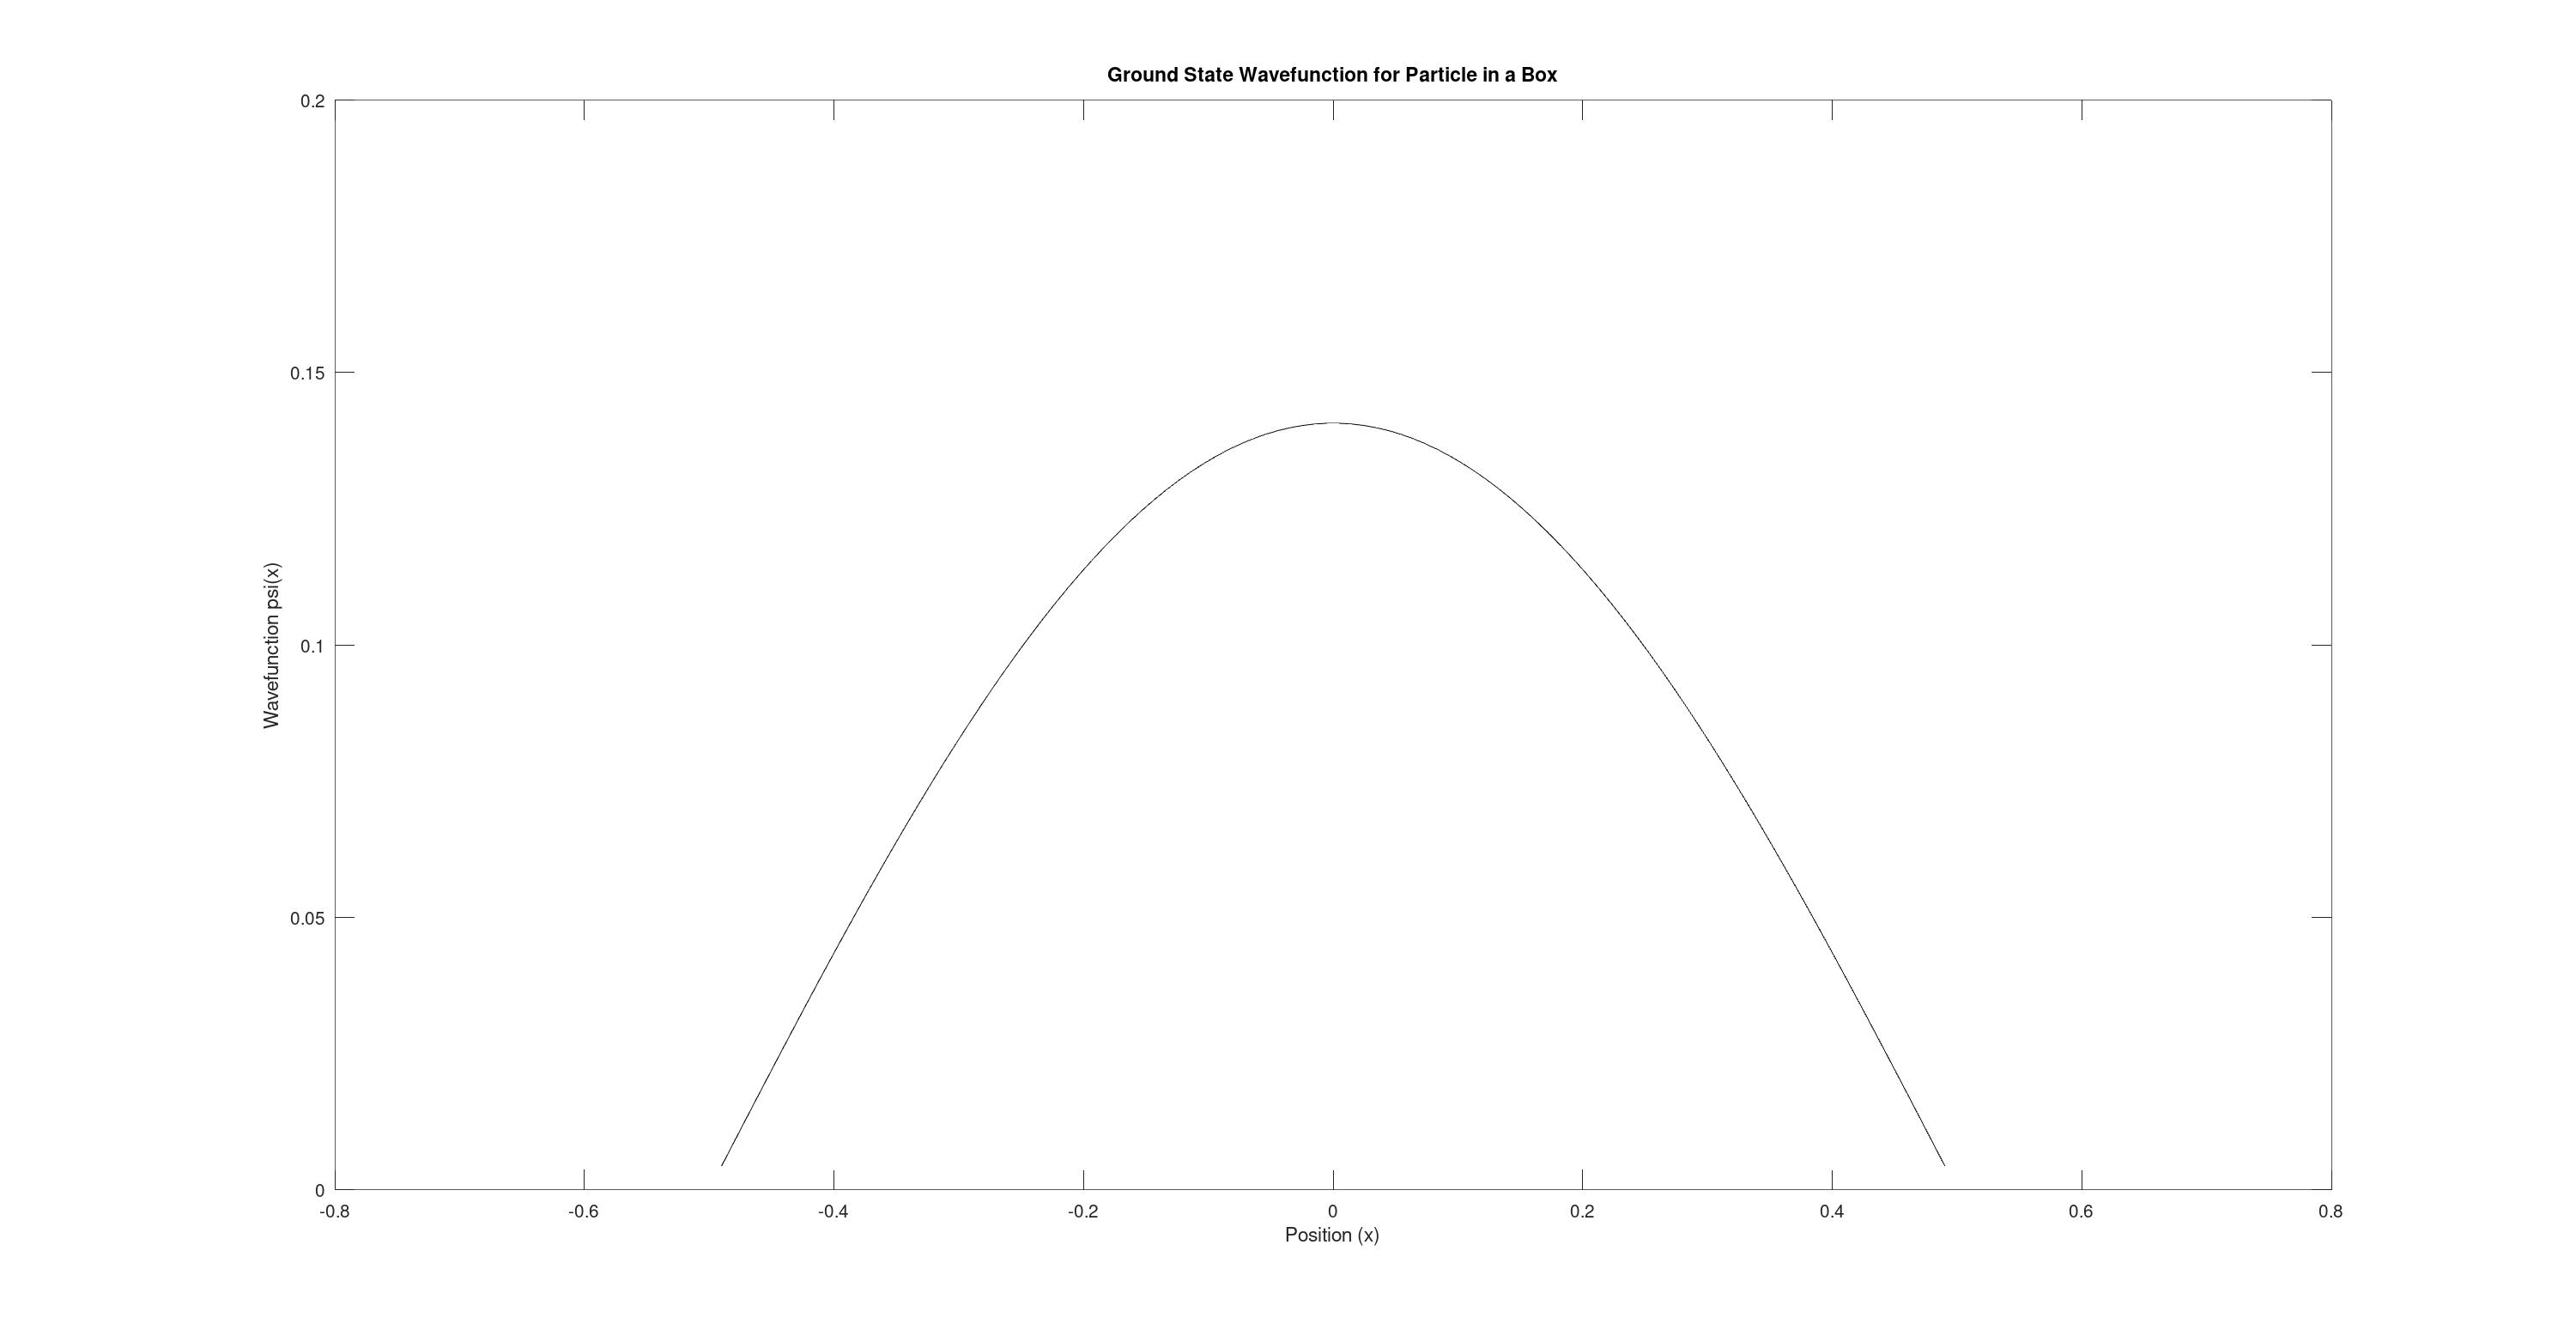
\includegraphics[width=1.0\textwidth]{a3.jpg}
  \caption{Normalized eigenfunction $\psi(x)$ obtained using shifted inverse iteration.}
  \label{fig:a3}
\end{figure}

\section*{Conclusion}
The shifted inverse iteration method successfully computes the ground state energy and eigenfunction of the discretized Hamiltonian. The method converges rapidly when the shift $\sigma$ is chosen close to the target eigenvalue. This approach demonstrates the utility of iterative solvers combined with Cholesky decomposition in quantum eigenvalue problems, particularly for large sparse systems.
